\section{模型建立与求解}

\subsection{问题一}

\subsubsection{模型的构建和分析}

在开始之前,我们需要先构建整个装置的物理模型。
以海平面为参考系。

当装置在水中静止时,对质量为 $m$ 的振子进行受力分析,则其受到的重力和受到弹簧弹力合力为零。
记以铅直向上为正方向,重力加速度为 $g$,记此时振子位移为 0,记此时弹簧压缩量为 $x_0$,弹簧的刚度为 $k$,则有 
\begin{equation}
    kx_0-mg=0 
    \label{oscilator}
\end{equation}

考虑在 $t$ 时刻,浮子位移 $x_1$,振子位移 $x_2$,正方向同前定义。
记阻尼器的阻尼系数为 $c$,对振子受力分析,如图 \ref{force-analysis} 左所示。我们有
\begin{equation}
    m\dfrac{\dif^2x_2}{\dif t^2}=k(x_1-x_2+x_0)+c(\dfrac{\dif{x_1}}{\dif{t}}-\dfrac{\dif{x_2}}{\dif{t}})-mg
\end{equation}
其中,$\dfrac{\dif^2 x_i}{\dif t^2}$ 即为瞬时加速度,$\dfrac{\dif x_i}{\dif t}$ 即为瞬时速度。

与此同时,我们对浮子进行受力分析,如图 \ref{force-analysis} 右所示。
记海水的兴波阻尼系数为 $c_0$,附加质量为 $m_0$,浮子质量为 $M$,波浪激励力为 $F$,有 
\begin{equation}
    M\dfrac{\dif^2x_1}{\dif t^2}=F+F_\text{浮}-Mg-k(x_1-x_2+x_0)-c(\dfrac{\dif{x_1}}{\dif{t}}-\dfrac{\dif{x_2}}{\dif{t}})-c_0\dfrac{\dif{x_1}}{\dif{t}}-m_0\dfrac{\dif^2 x_1}{\dif x_1^2}
\end{equation}

\begin{figure}[htbp]
    \centering
    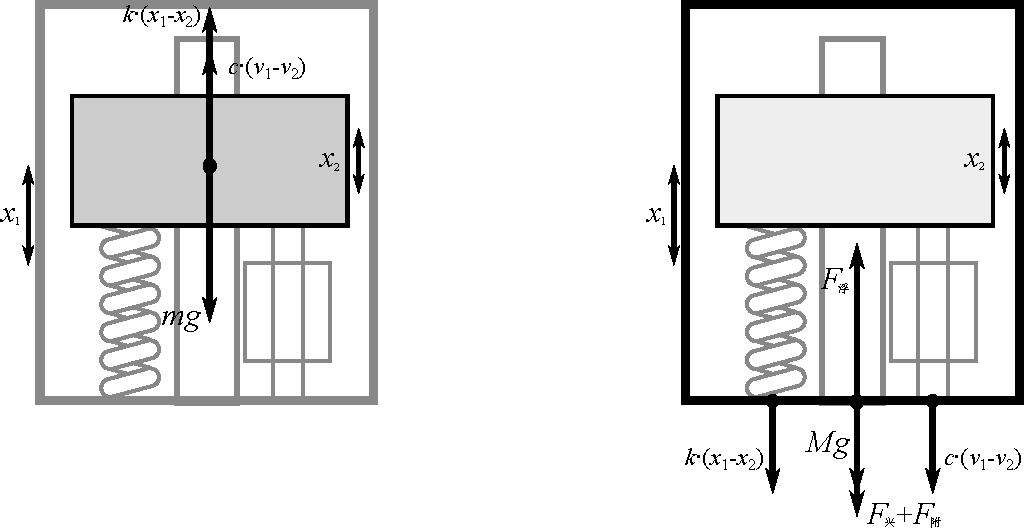
\includegraphics[width=11cm]{fig/force-analysis.pdf}
    \caption{对振子和浮子进行受力分析。为制图方便,未画出完整的浮子壳体}
    \label{force-analysis}
\end{figure}

我们需要确定起始时装置的深度。
记装置静止时受到的总浮力为 $F_\text{浮总}$,水的密度为 $\rho$,装置在水中漂浮时排水体积为 $V_\text{排总}$,则有
\begin{equation}
    \left\{
    \begin{aligned}
        & F_\text{浮总}=\rho gV_\text{排总} \\
        & (m+M)g=F_\text{浮总}
    \end{aligned}
    \right.
    \label{floating-relationship}
\end{equation}
代入附件 4 的数据容易求得 $V_\text{排总}\approx7.121\,\mathrm{m}^3$。
另一方面,考虑浮子下方锥体的体积,有 $V_\text{锥}=\dfrac{1}3\uppi r^2h\approx0.837\,\mathrm{m}^3$。显然,水没过了整个锥体部分,水面在浮子的柱体部分。此时,浮子因在液面中上升下降所造成的浮力变化 $\Delta F_\text{浮}=\rho g\Delta V_{排}=\rho gA\Delta x_1$,其中 $\Delta x_1$ 为浮子没入液面深度的变化量,$A$ 是圆柱的横截面面积。
从而有
\begin{equation}
    F_\text{浮}=F_\text{浮总}+\Delta F_\text{浮}=F_\text{浮总}-\rho gAx_1
    \label{floating}
\end{equation}

联立 \eqref{oscilator}—\eqref{floating} 式,我们可以消去 $mg$、$Mg$、$F_\text{浮}$ 和 $x_0$ 几项,得到
\begin{equation}
    \left\{
    \begin{aligned}
        &  m\dfrac{\dif^2x_2}{\dif t^2}=k(x_1-x_2)+c(\dfrac{\dif{x_1}}{\dif{t}}-\dfrac{\dif{x_2}}{\dif{t}}) \\
        &  M\dfrac{\dif^2x_1}{\dif t^2}=F-k(x_1-x_2)-c(\dfrac{\dif{x_1}}{\dif{t}}-\dfrac{\dif{x_2}}{\dif{t}})-\rho gAx_1-c_0\dfrac{\dif{x_1}}{\dif{t}}-m_0\dfrac{\dif^2 x_1}{\dif t^2}
    \end{aligned}
    \right.
    \label{chui-dang}
\end{equation}
式 \eqref{chui-dang} 就是关于浮子和振子垂荡运动的微分方程组。
考虑装置启动前静止,$t=0$ 时,有初值
\begin{equation}
    \left\{
    \begin{aligned}
        & x_1=x_2=0 \\
        & \dfrac{\dif x_1}{\dif t}=\dfrac{\dif x_2}{\dif t}=0
    \end{aligned}
    \right.
\end{equation}
求解这个初值问题,我们就能解出此题。

\subsubsection{问题求解}

根据附件 3 和附件 4,我们查得式 \eqref{chui-dang} 中的各个常数值如表 \ref{consts-1} 所示。
\begin{table}[htbp]
    \centering
    \begin{tabular}{cc}
        \toprule
        符号 & 常数的值 \\
        \midrule
        $M$ & \N{4866}\,kg \\
        $m$ & \N{2433}\,kg \\
        $k$ & \N{80000}\,$\mathrm{N}/\mathrm{m}$ \\
        $\rho$ & \N{1025}\,$\mathrm{kg}/\mathrm{m}^3$ \\
        $g$ & \N{9.8}\,$\mathrm{m}/\mathrm{s}^2$ \\
        $A$ & $\uppi\,\mathrm{m}^2$ \\
        $c_0$ & \N{656.3616}\,$\mathrm{N}\cdot\mathrm{s}/\mathrm{m}$ \\
        $m_0$ & \N{1335.535}\,kg \\
        \bottomrule
    \end{tabular}
    \caption{问题一适用的常量值}
    \label{consts-1}
\end{table}

同时,对于波浪激励力 $F$ 我们有
\begin{equation}
    F=f\cos(\omega t)
\end{equation}
其中 $f=\N{6250}\,\mathrm{N}$,$\omega=\N{1.4005}\,\mathrm{s}^{-1}$。
而对于阻尼系数 $c$,有
\begin{equation}
    c=\left\{
        \begin{aligned}
            & \N{10000}\,\mathrm{N}\cdot\mathrm{s}/\mathrm{m}, \text{对于情况 1} \\
            & \N{10000}\sqrt{\left|\dfrac{\dif x_1}{\dif t}-\dfrac{\dif x_2}{\dif t}\right|}\,\mathrm{N}\cdot(\mathrm{s}/\mathrm{m})^{3/2}, \text{对于情况 2}
        \end{aligned}
    \right.
\end{equation}

我们使用计算机对这个二元二阶线性初值问题进行数值求解。
对于题设的两种情况,我们均设定求解起点和终点为 0\,s 和 180\,s,以 0.2\,s 为间隔进行求解,得到在这 180\,s(即前 40 个周期)中,振子和浮子各自的位移和速度,如图所示。

完整的求解结果,我们已经存放在 \verb|result1-1.xlsx| 和 \verb|result1-2.xlsx| 文件中。其中,10\,s,20\,s,40\,s,60\,s,100\,s 时的数据如表 \ref{answer-1-1} 和表 \ref{answer-1-2} 所示。
\begin{table}[htbp]
    \centering
    \begin{tabular}{ccccccc}
        \toprule
        & & 10\,s & 20\,s & 40\,s & 60\,s & 100\,s \\
        \midrule
        \multirow{2}{*}{浮子} & 速度/$\mathrm{m}\cdot\mathrm{s}^{-1}$ & \N{-0.64101} & \N{-0.24095} & \N{0.31297} & \N{-0.47946} & \N{-0.60421} \\
        & 位移/$\mathrm{m}$ & \N{-0.19071} & \N{-0.59068} & \N{0.28538} & \N{-0.31450} & \N{-0.08361} \\
        \multirow{2}{*}{振子} & 速度/$\mathrm{m}\cdot\mathrm{s}^{-1}$ & \N{-0.69395} & \N{-0.27278} & \N{0.33291} & \N{-0.51573} & \N{-0.64300} \\
        & 位移/$\mathrm{m}$ & \N{-0.21168} & \N{-0.63425} & \N{0.29650} & \N{-0.33143} & \N{-0.08407}  \\
        \bottomrule
    \end{tabular}
    \caption{当 $c$ 为定值时,求解得到几个特殊时刻的浮子、振子位移和速度数据}
    \label{answer-1-1}
\end{table}

\begin{table}[htbp]
    \centering
    \begin{tabular}{ccccccc}
        \toprule
        & & 10\,s & 20\,s & 40\,s & 60\,s & 100\,s \\
        \midrule
        \multirow{2}{*}{浮子} & 速度/$\mathrm{m}\cdot\mathrm{s}^{-1}$  & \N{-0.64462} & \N{-0.24559} & \N{0.30628} & \N{-0.48281} & \N{-0.60582} \\
        & 位移/$\mathrm{m}$ & \N{-0.19199} & \N{-0.59419} & \N{0.28221} & \N{-0.31723} & \N{-0.08482} \\
        \multirow{2}{*}{振子} & 速度/$\mathrm{m}\cdot\mathrm{s}^{-1}$ &  \N{-0.70174} & \N{-0.28171} & \N{0.325991} & \N{-0.52082} & \N{-0.64558} \\
        & 位移/$\mathrm{m}$ & \N{-0.21378} & \N{-0.64018} & \N{0.29403} & \N{-0.33561} & \N{-0.08625} \\

        \bottomrule
    \end{tabular}
    \caption{当 $c$ 与相对速度相关时,求解得到几个特殊时刻的浮子、振子位移和速度数据}
    \label{answer-1-2}
\end{table}



\subsection{问题二}

\subsubsection{输出功率的推导}

波浪能系统的输出功率来自于 PTO 的阻尼力做功。
在 $t$ 时刻,设 PTO 的阻尼力为 $F_\text{PTO}$,记瞬时输出功率为 $P(t)$,则
    \begin{align}
        & F_\text{PTO}=c|v_1-v_2| \\
        & P(t)=F_\text{PTO}\Delta v=c(v_1-v_2)^2
    \end{align}
其中 $v_1$、$v_2$ 是浮子和振子的速度。
得到瞬时功率之后,将其在一段时间内累加(积分)并取平均值,即可得到平均输出功率
\begin{equation}
    \bar{P}=\dfrac{1}{T}\int\limits_0^TP(t)\dif t\approx\dfrac{1}{T}\sum_{i=1}^n\dfrac{P(t_i)+P(t_{i+1})}{2}\Delta t
\end{equation}
结合问题一的方法计算离散的速度、位移与时间的关系,我们容易算出给定条件下的 PTO 输出功率。

\subsubsection{最优参数的选择}

本题需要找出在 (1) $c$ 为常数且 $c\in[0, \N{100000}]\,(\mathrm{N}\cdot\mathrm{s}/\mathrm{m})$ 和 (2) $c=C|v_1-v_2|^p$,其中 $C\in[0, \N{100000}]\,(\mathrm{N}\cdot(\mathrm{s}/\mathrm{m})^{p+1})$ 和 $p\in[0, 1]$ 为常数的两种情况下,平均输出功率 $\bar{P}$ 的最大值和相应的常数系数。
本问题使用的与问题一所不同的量如表 \ref{consts-2} 所示。
\begin{table}[htbp]
    \centering
    \begin{tabular}{cc}
        \toprule
        符号 & 量的值 \\
        \midrule
        $F$ & $f\cos(\omega t)$,其中 $f=\N{4890}\,\mathrm{N}$,$\omega=\N{2.2143}\,\mathrm{s}^{-1}$ \\
        $c_0$ & $\N{167.8395}\,\mathrm{N}\cdot\mathrm{s}/\mathrm{m}$ \\
        $m_0$ & $\N{1165.992}\,\mathrm{kg}$ \\
        \bottomrule
    \end{tabular}
    \caption{问题二使用的与问题一不同的量}
    \label{consts-2}
\end{table}

对于传统的连续解析函数的极(最)值优化问题,我们有诸如爬山法、梯度下降法、Adams 算法等多种方法。
然而,这些方法都依赖函数的可导性质。
在问题一中,我们得到的是离散的点集,显然传统的函数优化方法不再适用。
为了高效地找到其中的最优化值,我们使用一种类似「随机梯度下降」的方法进行函数优化。


我们将上面的过程编写为 Python 程序并运行,最终运行得到的优化结果如表 \ref{answer-2-1} 和 \ref{answer-2-2} 所示。
\begin{table}[htbp]
    \centering
    \begin{tabular}{cc}
        \toprule
        输出功率/W & 阻尼系数/$\mathrm{N}\cdot\mathrm{s}/\mathrm{m}$ \\
        \midrule
        1 & 2 \\
        \bottomrule
    \end{tabular}
    \caption{输出功率的最大值,以及此时的阻尼系数}
    \label{answer-2-1}
\end{table}

\begin{table}[htbp]
    \centering
    \begin{tabular}{ccc}
        \toprule
        输出功率/W & 比例系数/$\mathrm{N}\cdot(\mathrm{s}/\mathrm{m})^{p+1}$ & 幂指数 \\
        \midrule
        1 & 2 & 3 \\
        \bottomrule
    \end{tabular}
    \caption{输出功率的最大值,以及此时的阻尼系数}
    \label{answer-2-2}
\end{table}

同时,为了直观验证结果的合理性,我们也使用 Wolfram Engine 内置的点集绘图功能,绘制了平均输出功率 $P$ 与阻尼系数、比例系数、幂指数等的关系图。
对于情况 1,关系如图 \ref{result-2-1} 所示,而对于情况 2,关系如图 \ref{result-2-2} 所示。
不难发现,我们使用算法得到的优化解,与图上所显示出的走向趋势一致。

\subsection{问题三}

\subsubsection{运动方程的建立}

与问题一相比,问题三加入了中轴的旋转,使得整个系统的运动变得复杂。
我们有必要建立新的细化的物理模型,从而列出新的运动方程。

本问题的模型中,外部浮子有两种不同类型的运动:一种是在竖直方向波浪激励力的作用下,在铅直方向进行的直线运动;另一种是在波浪激励力矩的影响下,绕某个轴进行的转动。
而在浮子的内部,振子由 PTO 和中轴所约束,PTO 和中轴的根部用一绞链与浮子相连结,亦绕绞链所在轴进行转动。
为了便于问题的分析,我们拟定下面的前提:
\begin{enumerate}
    \item 浮子的转动是绕其质心进行的定轴转动,振子的转动中心则是中轴与中轴底座绞接处。中轴底座、转轴等结构的厚度为零。
    \item 题目中所提供的波浪激励力矩 $L\cos(\omega t)$ 可视为力偶矩,它不为浮子的平动提供加速度。
\end{enumerate}

我们以整个装置静止直立在水面上时,浮子的质心为原点,以来流指向方向为 $x$ 轴正方向,以铅直向上为 $z$ 轴正方向,建立空间直角坐标系 $O-xyz$。
在装置运行的某一时刻 $t$,在 $xOz$ 投影面上装置的运行状态如图 \ref{status} 所示。
\begin{figure}[htbp]
    \centering
    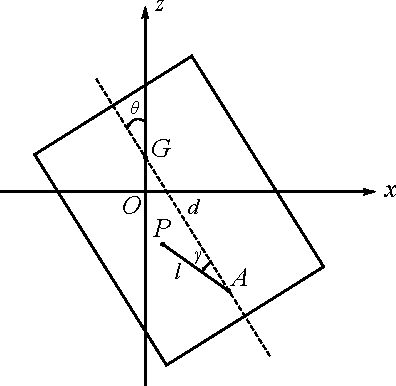
\includegraphics[width=6cm]{fig/problem-3-1.pdf}
    \caption{某时刻,$xOz$ 投影面上的装置运行状态}
    \label{status}
\end{figure}

在图中,$G$ 是浮子的质心。
显然,浮子是一个对称旋转体,故 $G$ 始终位于浮子的旋转轴(图中的虚线)上。
$A$ 点是绞链所在的点,由题目条件知道绞接处也位于浮子的旋转轴上。
$P$ 点是振子质心所在的点,$AP$ 连线表示的就是 PTO 和中轴构成的结构。
考虑装置中所有的转动,我们记 $\theta$ 为浮子的纵摇角,记 $\gamma$ 为振子相对于浮子的纵摇角,角度以图上视角逆时针为正值。
同时,为了便于分析,我们记 $l$ 为弹簧在此时的长度,记 $d$ 为线段 $AG$ 的长度,即转轴绞接处与浮子质心的距离。

方便起见,我们设此时 $G$ 点的坐标为 $(x_G, 0, z_G)$,设此时 $P$ 点的坐标为 $(x_P, 0, z_P)$。
对振子进行受力分析。
振子在水平和竖直方向产生的加速度分别为 $\dfrac{\dif^2 x_P}{\dif t^2}$ 和 $\dfrac{\dif^2 z_P}{\dif t^2}$,而振子受到的外力有 PTO 装置(弹簧和阻尼器)的推拉力 $F_\text{PTO}$、振子自身重力 $mg$ 以及其受到中轴(视为轻杆)的支持力 $F_{AB}$。
在 $x$ 和 $z$ 方向分别列出振子的运动学方程,有
\begin{align}
    m\cdot\dfrac{\dif^2 x_P}{\dif t^2} &= -F_\text{PTO}\sin(\theta+\gamma)+F_{AB}\cos(\theta+\gamma) \label{problem-3-eq1}\\
    m\cdot\dfrac{\dif^2 z_P}{\dif t^2} &= F_\text{PTO}\cos(\theta+\gamma)-mg+F_{AB}\sin(\theta+\gamma)
\end{align}

考虑振子的转动,设其在弹簧长度为 $l$ 时的转动惯量为 $I_B(l)$。
以逆时针为正方向。
记绞接处旋转阻尼器产生的旋转力矩为 $M_\text{PTO}$,则可以列出如下的转动运动学方程
\begin{equation}
    I_B(l)\cdot\dfrac{\dif^2(\theta+\gamma)}{\dif t^2}=M_\text{PTO}-F_{AB}\cdot l
\end{equation}

再来分析浮子。
% 在水平方向,由前文的前提分析可知,浮子受到的合力为零。
% 而在这一方向能产生分力的,只有 $F_{ABx}$ 和 $F_\text{PTO}$ 的反作用力。
% 我们容易得到
% \begin{equation}
%     F_\text{PTO}\sin(\theta+\gamma)-F_{ABx}=0
% \end{equation}
在水平方向,浮子只受到 $F_\text{PTO}$ 和 $F_{AB}$ 的水平分力,故有
\begin{equation}
    M\cdot\dfrac{\dif^2 x_G}{\dif t^2}= F_\text{PTO}\sin(\theta+\gamma)-F_{AB}\cos(\theta+\gamma)
\end{equation}
而在竖直方向,浮子受到波浪激励力 $F$、自身重力 $Mg$、PTO 反作用力 $F_\text{PTO}$ 的竖直分力、杆支持力的反作用力 $F_{AB}$ 的水平竖直分力,以及浮力(静水恢复力) $F_\text{浮}$、附加惯性力 $m_0\dfrac{\dif^2z_G}{\dif t^2}$、兴波阻尼力 $c_0\dfrac{\dif z_G}{\dif t}$。
因此有
\begin{equation}
    M\cdot\dfrac{\dif^2 z_G}{\dif t^2}=F+F_\text{浮}-Mg-F_\text{PTO}\cos(\theta+\gamma)-F_{AB}\sin(\theta+\gamma)-m_0\dfrac{\dif^2z_G}{\dif t^2}-c_0\dfrac{\dif z_G}{\dif t}
\end{equation}

最后,我们分析浮子的转动过程。
记波浪激励力矩为 $M_\text{wave}$,浮子绕过其质心的轴的转动惯量为 $I_A$,附加转动惯量为 $I_0$,兴波阻尼力矩系数为 $c_\text{r0}$,静水恢复力矩系数为 $M_\text{rec}$,有
\begin{equation}
    I_A\dfrac{\dif^2\theta}{\dif t^2}=M_\text{wave}-M_\text{PTO}-F_{AB}\cos(\theta+\gamma)\cdot d\cos\theta-F_{AB}\sin(\theta+\gamma)\cdot d\sin\theta-I_0\dfrac{\dif^2\theta}{\dif t^2}-c_\text{r0}\dfrac{\dif\theta}{\dif t}-M_\text{rec}\theta \label{problem-3-eq5}
\end{equation}

式 \eqref{problem-3-eq1}—\eqref{problem-3-eq5} 构成一组微分方程组。
其中的未知函数是 $\theta$、$\gamma$、$l$、$z_G$、$x_G$ 和 $F_{AB}$,它们都是时间 $t$ 的函数。
下面,我们尝试确定上述方程中的系数和常数,从而使得微分方程可以被解算。

\subsubsection{参数的求值}

考虑弹簧和阻尼器构成的 PTO。
容易知道
\begin{equation}
    F_\text{PTO}=-k(l-l_0)-c\dfrac{\dif l}{\dif t}
\end{equation}

考虑转轴绞接处的旋转 PTO,记扭转弹簧的刚度系数为 $k_\text{rot}$,旋转阻尼器的阻尼系数为 $c_\text{rot}$,有
\begin{equation}
    M_\text{PTO}=-k_\text{rot}\gamma-c_\text{rot}\dfrac{\dif \gamma}{\dif t}
\end{equation}

考虑几何关系,有
\begin{align}
    x_P&=x_G+d\sin\theta-l\sin(\theta+\gamma) \\
    z_P&=z_G-d\cos\theta+l\cos(\theta+\gamma)
\end{align}

考虑浮子的质心 $G$。
显然浮子是由一个无底圆锥面、一个圆柱侧面和一个圆面构成的组合体,对此组合体的各个部分求质心,我们容易求得此组合体的质心距离圆锥部分顶点的长度为 $d_G\approx\N{2.20792}\,\mathrm{m}$。
故 $d=d_G-\N{0.8}\,\mathrm{m}=\N{1.40792}\,\mathrm{m}$。

考虑浮子在做摇荡运动时的的排水量变化。
如图 \ref{floating-fig} 所示,设原先质心位置为 $G_0$,现在质心位置为 $G$,浮子角度为 $\theta$。
为了计算当前浮子排水的体积,我们可以延长 $GG_0$ 和 $AG$ 到海平面,容易知道 $BG=\dfrac{d_G}{\cos\theta}$。
因此 $AB=AG+GB$ 可以容易算出。
另一方面,由对称性可知 $V_A=V_B$,因此排水体积即为 $B$ 点之下浮子的体积。
代入数据得
\begin{equation}
    V_\text{排}=\N{5.2609}+\N{1.86007}\sec \theta-\uppi z_G\sec \theta
\end{equation}

\begin{figure}[htbp]
    \centering
    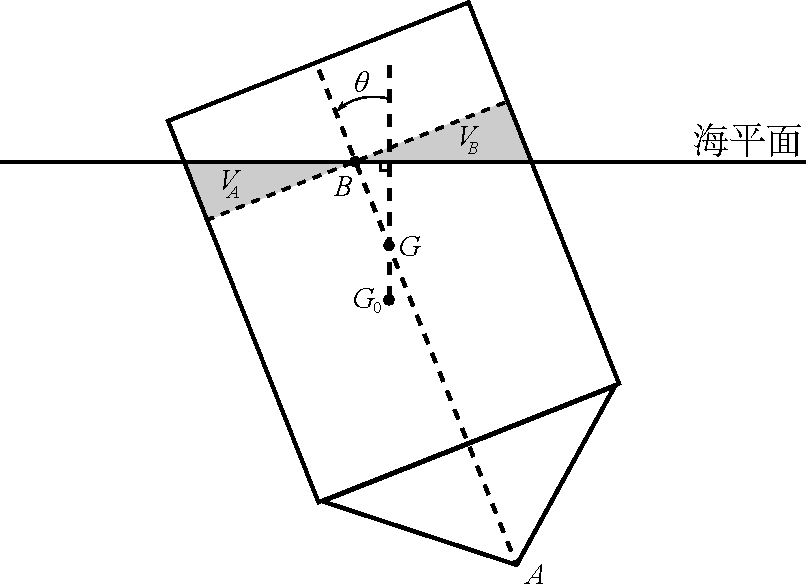
\includegraphics[width=8cm]{fig/floating.pdf}
    \caption{浮子排水量计算示意}
    \label{floating-fig}
\end{figure}

考虑浮子绕重心做纵摇运动的转动惯量,易知该浮子可以看成是由一个无底圆锥面、一个圆柱侧面和一个圆面的组合体。
容易知道
\begin{equation}
    I_A=I_\text{锥}+I_\text{柱}+I_\text{圆}
\end{equation}
我们先考虑一个理想均匀细圆环绕一平行于其直径的转轴旋转时的转动惯量。
记圆环半径为 $R$,转轴到圆环所在平面距离为 $l$。
取圆环上 $\dif\theta$ 角对应的一小段,其长度为 $R\dif\theta$。
若圆环线密度为 $\lambda$,则这段圆环的转动惯量
\begin{equation}
    \dif I=\lambda\cdot R\dif\theta(l^2+R^2\cos^2\theta)
\end{equation}
所以对整个环有
\begin{equation}
    I_\text{ring}=\int\limits_0^{2\uppi}\lambda R\dif\theta(l^2+R^2\cos^2\theta)
\end{equation}
圆锥面、圆柱面和圆盘都可以分解为圆环在特定方向上的积分。
对圆锥,记半顶角大小为 $\delta$,有
\begin{equation}
    \begin{aligned}
        I_\text{锥} &= \int\limits_0^{h_\text{锥}}I_\text{ring}\dif p \\
        &=\int\limits_0^{h_\text{锥}}\dfrac{1}{\cos\delta}\dif p\int\limits_0^{2\uppi}\rho p\tan\delta((\d_G-p)^2+(p\tan\delta)^2\cos^2\theta)\dif\theta
    \end{aligned}
\end{equation}
同理对圆柱有
\begin{equation}
        I_\text{柱} = \int\limits_{h_\text{柱底}}^{h_\text{柱顶}}\dif p\int\limits_{0}^{2\uppi}\rho R(p^2+R^2\cos^2\theta)\dif\theta
\end{equation}
对圆面有
\begin{equation}
    I_\text{圆} = \int\limits_0^R\dif p\int\limits_0^{2\uppi}\rho p(l^2+p^2\cos^2\theta)\dif\theta
\end{equation}
我们代入相应的尺寸数据,得到
\begin{equation}
    I_A=\N{8399.2}\,\mathrm{kg}\cdot\mathrm{m}^2
\end{equation}

另一方面,我们考虑振子绕转轴转动的转动惯量,有转轴绞接处到振子底部圆心的距离为 $l$。
设振子圆柱体厚度为 $h$,半径为 $r$,有
\begin{equation}
        I_B(l) =\dfrac{(4h^2-12h(h+l)+3r^2+12(h+l)^2)m}{12} 
        \label{last-eq-3}
\end{equation}    

联立式 \eqref{problem-3-eq1}—\eqref{last-eq-3},可以得到一组有六个未知函数的微分方程。

\subsubsection{数值求解}

对于问题三,我们使用的常量如表 \ref{consts-3} 所示。

\begin{table}[htbp]
    \centering
        \begin{tabular}{cc}
            \toprule
            符号 & 常数的值 \\
            \midrule
            $M$ & \N{4866}\,kg \\
            $m$ & \N{2433}\,kg \\
            $\rho$ & \N{1025}\,$\mathrm{kg}/\mathrm{m}^3$ \\
            $g$ & \N{9.8}\,$\mathrm{m}/\mathrm{s}^2$ \\
            $A$ & $\uppi\,\mathrm{m}^2$ \\
            $k$ & \N{8000}\,$\mathrm{N}/\mathrm{m}$ \\
            $c$ & $\N{10000}\,\mathrm{N}\cdot\mathrm{s}/\mathrm{m}$ \\
            $k_\text{rot}$ & $\N{250000}\,\mathrm{N}\cdot\mathrm{m}$ \\
            $c_\text{rot}$ & $\N{1000}\,\mathrm{N}\cdot\mathrm{m}\cdot\mathrm{s}$ \\
            $l_0$ & $\N{0.5}\,\mathrm{m}$ \\
            $M_\text{rec}$ & $\N{8890.7}\,\mathrm{N}\cdot\mathrm{m}$ \\
            $m_0$ & $\N{1028.876}\,\mathrm{kg}$ \\
            $I_0$ & $\N{7001.914}\,\mathrm{kg}\cdot\mathrm{m}^2$ \\
            $c_0$ & $\N{683.4558}\,\mathrm{N}\cdot\mathrm{s}/\mathrm{m}$ \\
            $c_\text{r0}$ & $\N{655.3383}\,\mathrm{N}\cdot\mathrm{m}\cdot\mathrm{s}$ \\
            \bottomrule
        \end{tabular}    
        \caption{问题三适用的常量值}
        \label{consts-3}
\end{table}        

同时,本问题中使用的波浪激励力和力矩 $F$ 与 $M_\text{wave}$ 满足
\begin{equation*}
    \left\{
    \begin{aligned}
        & F=f\cos(\omega t) \\
        & M_\text{wave}=L\cos(\omega t) \\
        & f=\N{3640}\,\mathrm{N} \\
        & L=\N{1690}\,\mathrm{N}\cdot\mathrm{m} \\
        & \omega=\N{1.7152}\,\mathrm{s}^{-1} \\
    \end{aligned}    
    \right.
\end{equation*}    

将以上方程输入计算机中求解,可以得到各个时刻下浮子和振子的位移、速度、角位移、角速度,如图至图所示。
完整的求解结果,我们已经存放在 \verb|result3.xlsx|文件中。其中,10 s,20 s,40 s,60 s,100 s 时的数据如表 和表 所示。

\subsection{问题四}

\subsubsection{输出功率的推导}

问题四在问题二的基础上,增加了绕轴旋转的纵摇运动。
我们可以利用问题三已经计算出来的各个时刻的浮子、振子状态,来计算一系列瞬时功率并进行积分,即可求得平均功率。
